\section{Theorie}


In  dieser  Arbeit  geht  es  um die  Synthetisierung  und  Optimierung  eines
Mikrowellenfilters (Stubfilter) in Mikrostreifen-Technologie.

\begin{figure}[h!]
\centering
 	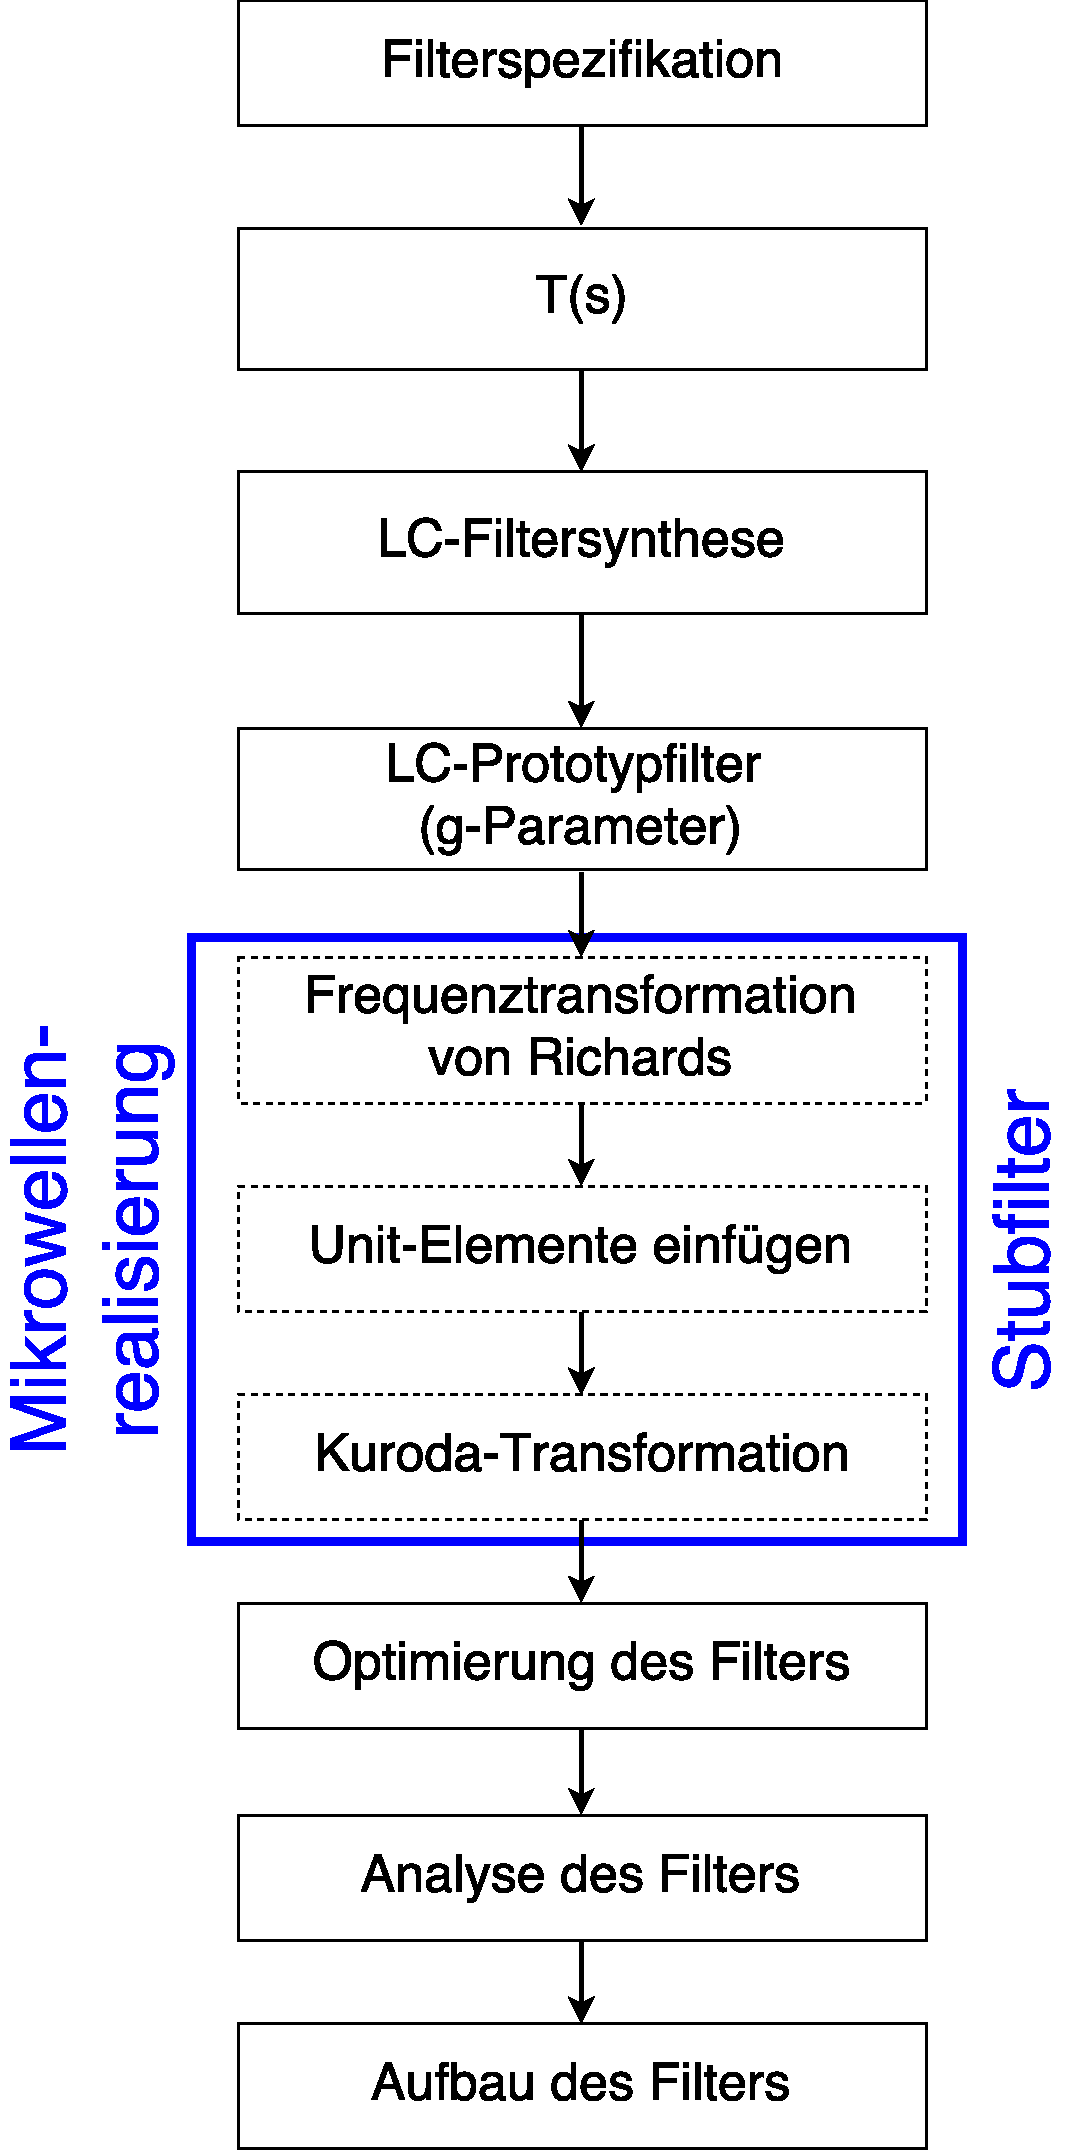
\includegraphics[width=\imagewidth]{images/Ablauf_Filterdimensionierung.pdf}
 	\caption{Ablauf Stubfilter-Dimensionierung}
 	\label{fig:Ablauf_Filterdimensionierung}
\end{figure}

Ausgangslage  für  die  Synthethisierung  des  Stubfilter  sind oftmals voberechnete
``g-Parameter'',  welche  nach  Methoden  der   klassischen  LC-Filtersynthese
gefunden  werden.  Diese  ``g-Parameter'' beschreiben  ein  impedanznormiertes
LC-Prototypfilter, auf    welches    zwei    verschiedene   Transformationen
angewendet werden: Die Richard's Transformation und die Kuroda Transformation.

Mit der Richard's Transformation können  die konzentrierten Elemente (L,C) des
Prototypfilters mit verteilte  Elementen  (Stubs)  ersetzt werden. Nach dieser
Transformation  spricht  man  von einem Stubfilter. Das Problem ist aber, dass
sich dieses Filter nicht realisieren lässt,  weil sich alle Stubs konzentriert
am gleichen Ort befinden.

Deshalb  wird  im Anschluss  die  Kuroda  Transformation  verwendet,  um  eine
physikalische Distanz zwischen den Stubs zu schaffen, damit das Filter auch in
Realit\"at  umgesetzt  werden  kann.  Obwohl  für  die  Kuroda  Transformation
sogenannte  ``Unit  Elements''  eingebaut  werden  müssen,  ändert   sich  das
Verhalten nicht.

Im  Anschluss  an   die  Filtersynthese  wird  der  Sperrbereich  des  Filters
optimiert,  was  eine  Erhöhung  der Filterordnung um die  Anzahl  eingebauter
``Unit  Elements'' bewirkt.

\subsection{Prototypfilter}

Bei jeder Filterdimensionierung wird von einem Prototypfilter ausgegangen, welches üblicherweise in der Form eines normierter Tiefpassfilters vorliegt. Abb.\ref{fig:Prototyp_Filter} zeigt die Topologie eines möglichen Tiefpassfilters (a) mit zugehöriger dualer Topologie (b).

\begin{figure}[h!]
\centering
 	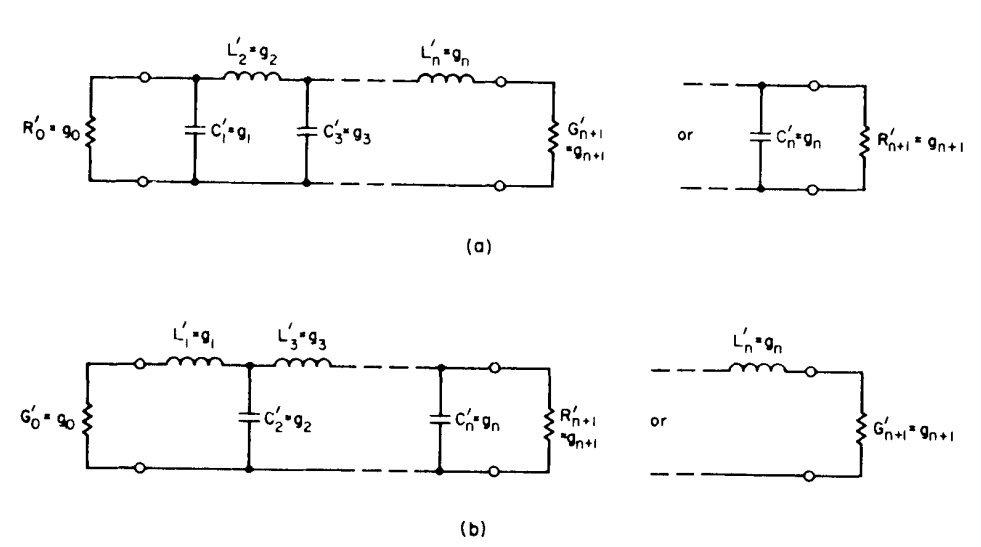
\includegraphics[width=0.5\textwidth]{Prototyp_Filter.png}
 	\caption{Prototypfilter (Tiefpass)}
 	\label{fig:Prototyp_Filter}
\end{figure}

%Quelle : Microwave Filters Impadance Matching Networks and Coupling Structures, P95, Fig4.04-1

Die Werte $g_0$ bis $g_{n+1}$ sind die Elementwerte des Protottypfilters. Diese Elementwerte können aus Tabellen entnommen werden und sind so normiert, dass das beschriebene  Prototypfilter die Grenzfrequenz $\omega_{C} = 1$, sowie die Lastimpedanz (oder Lastadmittanz) von $g_{n+1}=1\Omega$ aufweist. Dadurch kann der Prototyp sehr einfach in ein konkretes LC-Filter mit der gewünschten Lastimpedanz und Grenzfrequenz umgerechnet werden. 

Die Umrechnung in ein konkretes LC-Filter mit einer Lastimpedanz $Z_0$ und einer Grenzfrequenz $\omega_{C} = 1$ wird auch Entnormierung genannt und kann mit folgenden Formeln bewerkstelligt werden: 

\begin{equation}\label{eq:R}	
R_i = R'_i \cdot Z_0
\end{equation}

\begin{equation}\label{eq:L}	
L_i = \frac{L'_i \cdot Z_0}{\omega_{C}}
\end{equation}

\begin{equation}\label{eq:C}	
C_i = \frac{C'_i}{Z_0 \cdot \omega_{C}}
\end{equation}

Dabei beschreiben  $R'_i$, $C'_i$ und $L'_i$ die normierten Elementwerte  $g_0$ bis $g_{n+1}$ und $R_i$, $C_i$, und $L_i$ die konkreten Werte nach der Entnormierung.

\subsection{Stubfilter}

Im Kapitel \ref{sec:Protototypfilter} wurde gezeigt, wie durch die Entnormierung eines Prototypfilter ein konkretes LC-Filter dimensioniert werden kann. Solche LC-Filter  können in einem weiten Frequenzbereich  eingesetzt  werden.  Jedoch
wird  bei realen konzentrierten Elementen (R,L,C) zu höheren Frequenzen hin der Einfluss der parasitären Eigenschaften immer deutlicher, so dass hohe Anforderungen an die Bauteilgüte  gestellt  werden  müssen. Im GHZ-Bereich wird es daher  zunehmend attraktiv,  statt  konzentrierten  Kapazitäten  und  Induktivitäten  verteilte
Strukturen  in  Form  von  Leitungen  zu  verwenden.\cite[p.~203]{ref:gustrau}  Man  spricht   dann  von sogenannten Leitungsfiltern.



Es gibt verschiedene Arten um  Leitungsfilter zu realisieren. Eine Möglichkeit der  Realisierung  ist das Stubfilter.  Dieses  Filter  verwendet  gleichlange kurzgeschlossenen Leitungen (TLSC) und  leerlaufende  Leitungen(TLOC), welche an einem Ende verbunden und am anderen Ende entweder kurzgeschlossen
oder offen gelassen werden. Diese sogenannten Stubs oder Stichleitungen werden mit gleichlangen Verbindunsleitungen (TLIN) verbunden. 

In Abb. \ref{fig:Stubfilter} ist ein solches Stubfilter zu sehen, welches aus 8 kurgeschlossenen Stubs (TLSC) besteht.

\begin{figure}[h!]
\centering
 	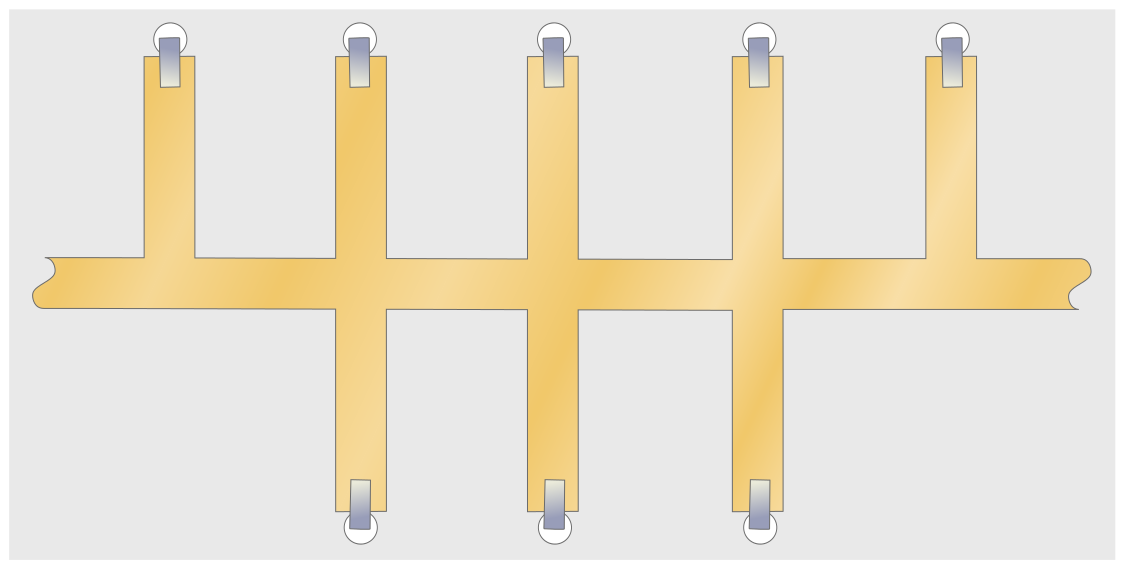
\includegraphics[width=\imagewidth]{images/Stripline_Stub_Filter}
 	\caption{Beispiel eines Stubfilters, Wikipedia \cite{ref:wikipedia:stripline}}
 	\label{fig:Stubfilter}
\end{figure}

Stubs verhalten sich bei  hohen  Frequenzen  wie  reaktive Elemente(L,C) und ermöglichen so die Realisierung  eines  Mikrowellenfilters. Für Stubfilter existiert eine geschlossene Thoerie zur Filtersynthese. Dadurch muss ein herrkömmliches Prototypfilter nur entnormiert und transformiert werden, um das gewünschte Stubfilter mit den gewünschten Eigenschaften zu erhalten.


\subsection{Richards Frequenztransformation}

Der  Frequenzbereich von konzentrierten LC-Filtern ist beschr\"ankt durch  die
Nichtidealit\"at der Komponenten.  W\"ahrend  die  Reaktanz und die G\"ute von
konzentrierten Induktivit\"aten und Kapazit\"aten  im  Bereich  \"uber  einige
\SI{100}{\mega\hertz} keinen hohen Filteranspr\"uchen mehr gen\"ugen k\"onnen,
w\"aren die entsprechenden Reaktanzen noch  sehr gut mit verteilten Elementen,
wie   leerlaufenden   und   kurzgeschlossenen  Leitungen  sowie  verschiedenen
gekoppelten   Leitungen  realisierbar.   Es   ist   beispielsweise   aus   der
Leitungstheorie  bekannt,  dass  leerlaufende  Leitungen   mit  einer  L\"ange
$l\le\frac{\lambda}{4}$   kapazitiv   und   kurzgeschlossene   Leitungen   mit
$l\le\frac{\lambda}{4}$  induktiv  sind.  Wir  k\"onnten damit die  induktiven
Reaktanzen und  die  kapazitiven  Suszeptanzen  mit  solchen Leitungselementen
ersetzen.

Eine Methode dies zu  erreichen  ist mithilfe der sogenannten \textit{Richards
Frequenztransformation}.   Dabei   ist   wichtig   zu   beachten   dass   alle
Leitungselemente  die  gleiche  L\"ange   $l$  haben  m\"ussen.  Sie  hat  die
allgemeine Form:

\begin{equation}
    \Omega = \frac{\Omega'}{\Omega'_c} = \frac{1}{\Omega'_c}\tan\frac{\pi f}{2f_0}
    \label{eq:richards}
\end{equation}

Dabei sind

\begin{tabular}{ll}
    $\Omega$    & normierte Frequenz des konzentrierten \\ 
                & Netzwerkes \\
    $\Omega'$   & reelle normierte Frequenz $\Omega' = \tan\frac{\pi f}{2f_0}$ \\
    $\Omega'_c$ & reelle normierte Durchlassfrequenz \\
                & $\Omega'_c = \tan\frac{\pi f_c}{2f_0}$ \\
\end{tabular}

F\"ur die Leitungselemente des Filters gelten

\begin{align}
    j\Omega\omega_cL_i &= jZ_{w_i}\tan\frac{\pi f}{4f_c} \\
    j\Omega\omega_cC_i &= jY_{w_i}\tan\frac{\pi f}{4f_c}
\end{align}

Dabei sind

\begin{tabular}{ll}
    $L_i$ und $C_i$         & die Induktivit\"aten und Kapazi\"aten \\
                            & des konzentrierten Filters. \\
    $Z_{w_i}$ und $Y_{w_i}$ & die Wellenimpedanzen und Wellen-\\
                            & admittanzen der kurzgeschlossenen \\
                            & und leerlaufenden Leitungen \\
                            & des Leitungsfilters. \\
\end{tabular}

Zur Visualisierung wurde mit MATLAB der  Amplitudengang  $T(s)$ eines analogen
Chebychev-Tiefpass-filters 3.  Ordnung  mit  der  Formel  $s  =  j\tan\frac{\pi
\omega}{2\omega_0}$ (Formel \ref{eq:richards}) transformiert. Das Resultat ist
in der Abbildung \ref{fig:richards-example} zu sehen.

\begin{figure}[h!]
    \centering
    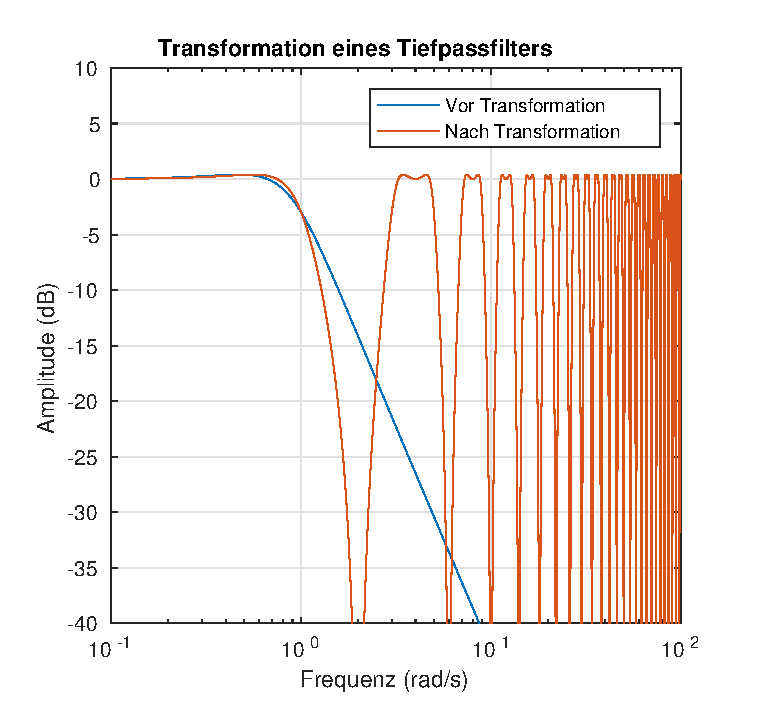
\includegraphics[width=\imagewidth]{images/richards-lowpass-example}
    \caption{Chebychev-Tiefpassfilters 3. Ordnung (blau) und die Richards-Transformierte davon (orange)}
    \label{fig:richards-example}
\end{figure}

Die  D\"ampfungscharakteristik  des   Leitungsfilters  weist  gegen\"uber  dem
konzentrierten  LC-Filter eine verzerrte Frequenzskala auf und ist  periodisch
mit der Periodizit\"at

\begin{equation}
    4f_c = \frac{\nu_p}{2l}
\end{equation}

Wobei $\nu_p$ die Phasengeschwindigkeit auf der Leitung ist.

Die Periodizit\"at war  zu  erwarten,  da  alle Leitungenselemente die gleiche
L\"ange $l$ haben.

\begin{figure}[h!]
    \centering
    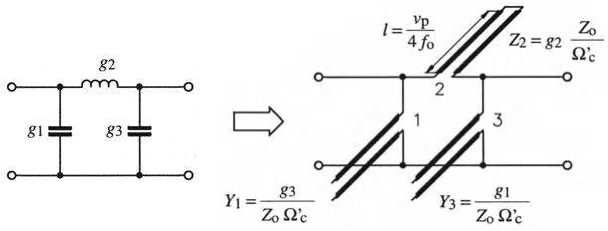
\includegraphics[width=\imagewidth]{images/LC-zu-Leitungsfilter}
    \caption{Realisierung von Stichleitungen in Mikrostreifentechnik, Auszug aus dem Buch Mikrowellentechnik\cite[p.~26]{ref:baechtold}}
    \label{fig:LC-zu-Leitungsfilter}
\end{figure}


\subsection{Kuroda Transformation}



